% This is "sig-alternate.tex" V2.0 May 2012
% This file should be compiled with V2.5 of "sig-alternate.cls" May 2012
%
% This example file demonstrates the use of the 'sig-alternate.cls'
% V2.5 LaTeX2e document class file. It is for those submitting
% articles to ACM Conference Proceedings WHO DO NOT WISH TO
% STRICTLY ADHERE TO THE SIGS (PUBS-BOARD-ENDORSED) STYLE.
% The 'sig-alternate.cls' file will produce a similar-looking,
% albeit, 'tighter' paper resulting in, invariably, fewer pages.
%
% ----------------------------------------------------------------------------------------------------------------
% This .tex file (and associated .cls V2.5) produces:
%       1) The Permission Statement
%       2) The Conference (location) Info information
%       3) The Copyright Line with ACM data
%       4) NO page numbers
%
% as against the acm_proc_article-sp.cls file which
% DOES NOT produce 1) thru' 3) above.
%
% Using 'sig-alternate.cls' you have control, however, from within
% the source .tex file, over both the CopyrightYear
% (defaulted to 200X) and the ACM Copyright Data
% (defaulted to X-XXXXX-XX-X/XX/XX).
% e.g.
% \CopyrightYear{2007} will cause 2007 to appear in the copyright line.
% \crdata{0-12345-67-8/90/12} will cause 0-12345-67-8/90/12 to appear in the copyright line.
%
% ---------------------------------------------------------------------------------------------------------------
% This .tex source is an example which *does* use
% the .bib file (from which the .bbl file % is produced).
% REMEMBER HOWEVER: After having produced the .bbl file,
% and prior to final submission, you *NEED* to 'insert'
% your .bbl file into your source .tex file so as to provide
% ONE 'self-contained' source file.
%
% ================= IF YOU HAVE QUESTIONS =======================
% Questions regarding the SIGS styles, SIGS policies and
% procedures, Conferences etc. should be sent to
% Adrienne Griscti (griscti@acm.org)
%
% Technical questions _only_ to
% Gerald Murray (murray@hq.acm.org)
% ===============================================================
%
% For tracking purposes - this is V2.0 - May 2012

\documentclass{sig-alternate}

\usepackage{subfigure}
\usepackage{amsmath}
\usepackage{algorithm}
\usepackage{algpseudocode}
\usepackage{varwidth}
\usepackage{listings}
\usepackage[usenames,dvipsnames]{color}
\usepackage{multirow}
\usepackage{array}
\newcommand{\ddx}[2]{ \frac{ \partial #1}{ \partial {#2} } }
\newcommand{\ddt}[1]{\partial_t #1}
\newcommand{\Grad}[1]{\nabla #1}
\newcommand{\Div}[1]{\Grad \cdot #1}
\newcommand{\Lap}[1]{\Delta #1}
\definecolor{light-gray}{gray}{0.95}

\makeatletter
\def\BState{\State\hskip-\ALG@thistlm}
\makeatother

\makeatletter
\let\OldStatex\Statex
\renewcommand{\Statex}[1][3]{%
  \setlength\@tempdima{\algorithmicindent}%
  \OldStatex\hskip\dimexpr#1\@tempdima\relax}
\makeatother

\newcommand{\kk}[1]{{\color{blue}{\it KK: #1}}}

\begin{document}

%% \title{A Sample {\ttlit ACM} SIG Proceedings Paper in LaTeX
%% Format\titlenote{(Does NOT produce the permission block, copyright information nor page numbering). For use with ACM\_PROC\_ARTICLE-SP.CLS. Supported by ACM.}}
%% \subtitle{[Extended Abstract]
%% \titlenote{A full version of this paper is available as
%% \textit{Author's Guide to Preparing ACM SIG Proceedings Using
%% \LaTeX$2_\epsilon$\ and BibTeX} at
%% \texttt{www.acm.org/eaddress.htm}}}

\title{
Efficient evaluation of threshold queries of derived fields in a numerical simulation database
}

\numberofauthors{3} 
\author{
\alignauthor Kalin Kanov \\
     \affaddr{Department of Computer Science} \\
     \affaddr{IDIES} \\
     \affaddr{Johns Hopkins University} \\
     \affaddr{Baltimore, MD 21218} \\
     \email{kalin@cs.jhu.edu}
\alignauthor Randal Burns \\
     \affaddr{Department of Computer Science} \\
     \affaddr{IDIES} \\
     \affaddr{Johns Hopkins University}\\
     \affaddr{Baltimore, MD 21218} \\
     \email{randal@cs.jhu.edu} 
\alignauthor Cristian C. Lalescu \\
     \affaddr{Department of Applied Mathematics and Statistics} \\
     \affaddr{IDIES} \\
     \affaddr{Johns Hopkins University} \\
     \affaddr{Baltimore, MD 21218} \\
     \email{clalesc1@jhu.edu}
}

\maketitle

\begin{abstract}
%Data-intensive architectures and compute clusters have been deployed to store, manage and provide public access to such datasets. 
%The systems built on top of these architectures, sometimes called virtual laboratories, usually do not support the analysis functionality that scientists are 
%interested in out of the box. Moreover, d
In this paper, we present a method for the efficient evaluation of threshold queries of derived fields for large numerical 
simulation datasets stored in a cluster of relational databases. 
%Such simulations are commonplace in the study of many different physical phenomena. 
The datasets produced by these simulations are in the TB and even PB ranges. 
Data-intensive computations that examine entire time-steps of the simulation data are impractical to perform
locally by the user, taking days or months to iterate over the entire dataset. 
The integrated method for the evaluation of threshold queries that we have developed achieves scalability through data-parallel execution
of the computations on the nodes of an analysis database cluster. 
We extend the scientific analysis environment with the introduction of an application-aware cache for query results, building on the concept of semantic caching.
The cache has little overhead and improves query performance by over an order of magnitude for queries that hit the cache.
Caching the results of threshold queries preserves both the I/O and computation effort used to obtain them.
In the case of computational turbulence, this allows scientists to quickly focus on the most intense events and interesting regions in any time-step or 
the dataset as a whole, which greatly speeds up the rate of scientific exploration and discovery. 
\end{abstract}

%% % A category with the (minimum) three required fields
\category{H.2.8}{Database Management}{Database Applications -- Scientific Databases}
\category{H.2.4}{Database Management}{Systems -- Distributed Databases}
\category{J.2}{Computer Applications}{Physical Sciences and Engineering -- Physics}

\keywords{scientific databases, data-intensive computing, threshold queries, turbulence} % NOT required for Proceedings

\vspace{10pt}
\section{Introduction}
%What is the problem?
Better instruments, faster and bigger supercomputers and easier collaboration and sharing of data in the sciences have introduced the need
to manage increasingly large datasets. Data-intensive systems and architectures have been developed with the goal of storing and providing
fast access to such datasets. Examples of such analysis environments include the GrayWulf and Data-Scope clusters \cite{Szalay, DataScope} at 
Johns Hopkins, which have capacity of 1.1PB and 11PB
respectively. One of their missions is to provide persistent storage and public access to world-class numerical simulation data. 
These systems differ from the traditional HPC environments in that they aim to achieve high aggregate throughput by balancing computation
capabilities with I/O and network bandwidth. The computing systems and services developed on top of these platforms are more than pure
storage engines and usually have complex analysis routines built-in, which has largely been driven by the ``move the computation to the data"
paradigm \cite{fourthparadigm}. These built-in analysis routines are most often not novel themselves. They implement core scientific functionality for the
study of the particular scientific phenomena, which was observed or simulated in the first place. The analysis routines however require novel evaluation
strategies and methods for their execution. They have to operate on large array datasets distributed across multiple nodes of a cluster of relational
databases. In order to reduce their running times, they have to make efficient use of the cluster resources and incorporate 
leading data management techniques.

Finding the locations or regions of highest vorticity or those with the largest norms of the velocity or other fields of interest
enables new insights in the study of fluid dynamics. Analysis of this kind coupled with the ability to analyze time-series datasets both 
forward and backward in time has transformed our understanding of turbulence \cite{Eyink}. Furthermore, threshold, top-$k$ queries and similarity search
in general are important in many different disciplines. We introduce an efficient evaluation strategy for threshold
queries over time-series datasets stored in a cluster of relational databases. Our method evaluates not only threshold queries of the vector or 
scalar field data stored in the database, but also performs thresholding of \emph{derived} fields. 

The main challenge that our approach tackles is that the
data-intensive computation of \emph{derived} fields has to be carried out on-demand for extremely large array datasets stored in an analysis cluster environment 
comprised of multiple database nodes. We focus on the evaluation of threshold queries of fields derived from the data stored in the cluster as
these queries are the most interesting scientifically. However, our approach applies to the evaluation of top-$k$ queries, rollup queries and data-reducing 
queries in general. The established data management techniques that our approach combines make the approach easy to understand. It can be applied to other 
scientific analysis environments, which manage large datasets in a database management system. Examples include the Sloan Digital Sky Survey
\cite{SDSS}, the Millennium Simulation \cite{Millennium} and the Open Connectome Project \cite{Burns}.

%Why is it hard? (E.g., why do naive approaches fail?)
Evaluating threshold queries within the database cluster allows scientists with modest computational and network capability to narrow down on and
examine some of the most interesting regions and features in the dataset and focus on the subsequent analysis needed to understand these events.
%The evaluation of threshold queries of derived fields requires a stencil kernel computation at each point on the grid in order to compute the field to be thresholded.
%The value of the derived field at each location depends on all the values at locations within the kernel of computation. 
%In order to evaluate such a query for a given time-step, all of the data for that time-step must be read and each data point 
%will appear in $N$ kernels of computation, in which $N$ is the size of the kernel. The evaluation is both data and computation intensive.
It is impractical to materialize all possible derived fields and store them alongside the raw data
due to the large size of the datasets and the limits of available storage.
Obtaining the derived field and thresholding locally by the user requires not only the computation of the derived field over an entire time-step server-side 
but also the transfer of a large amount of data over the network, most of which are subsequently discarded. 
One of our collaborators reported that such a local evaluation of a threshold
query over an entire time-step took over 20 hours. It would take months to iterate over the entire dataset. 
This highlighted the need for providing the capability through an integrated approach, which performs the evaluation server-side.

%It is impractical to materialize all possible derived fields and store them alongside the raw data
%due to the large size of the datasets and the limits of available storage. Therefore, the derived fields 
%have to be evaluated on-demand from the stored data and thresholding performed on the database nodes near the data.
%We will demonstrate that this integrated approach evaluates a threshold query over an entire time-step in a few minutes.

Database, operating and file system caches are effective at speeding up access to the large amounts of data stored on disk. However, this might not be
sufficient for some interactive applications, because these application-independent caches cannot exploit dataset-specific structure and applica\-tion-level
information \cite{Lopez}. Moreover, even if the data are available in one or more of these application-independent caches the computation associated 
with the derived field still needs to be performed for each point on the grid, because results of previous computations are not cached. 
We will demonstrate that an integrated approach, which computes the derived fields on-demand in a data-parallel manner, performs the evaluation over 
an entire time-step in a few minutes. Storing the query results in an application-aware semantic cache further reduces the running times to several 
seconds.

%Why is it interesting and important?
Thresholding allows scientists to obtain and examine the regions containing the most intense events and features in the dataset in the case of turbulence. 
These are often the locations that have the largest vorticity norms and have intense vortices or reconnection events. 
In magnetohydrodynamics, the locations of largest electric current are of great interest for similar reasons.
It is important that threshold queries are evaluated in an efficient manner, because often further subsequent examination
and analysis is required to understand the physics that drive these intense events. 

%Why hasn't it been solved before? (Or, what's wrong with previous proposed solutions? How does mine differ?)
There are several challenges that arise during the evaluation of threshold queries of derived fields in an analysis database cluster. The field variables have to be
evaluated \emph{on-demand} from the array data stored in the database cluster. The computations are data-intensive as they apply stencil kernels on extremely
large multidimensional array datasets. 
Stencil kernel computations have to be performed at each location on the grid as opposed to at a particular number of target locations. 
Each data point appears in $N$ kernels of computation, in which $N$ is the size of the kernel.
The evaluation needs to be distributed across the nodes of the database cluster to avoid the unnecessary movement of data over 
the network and to achieve scalability.
Techniques that target the traditional supercomputing environments do not translate directly to the 
distributed database setting of an analysis cluster environment. 

\begin{figure}
\centering
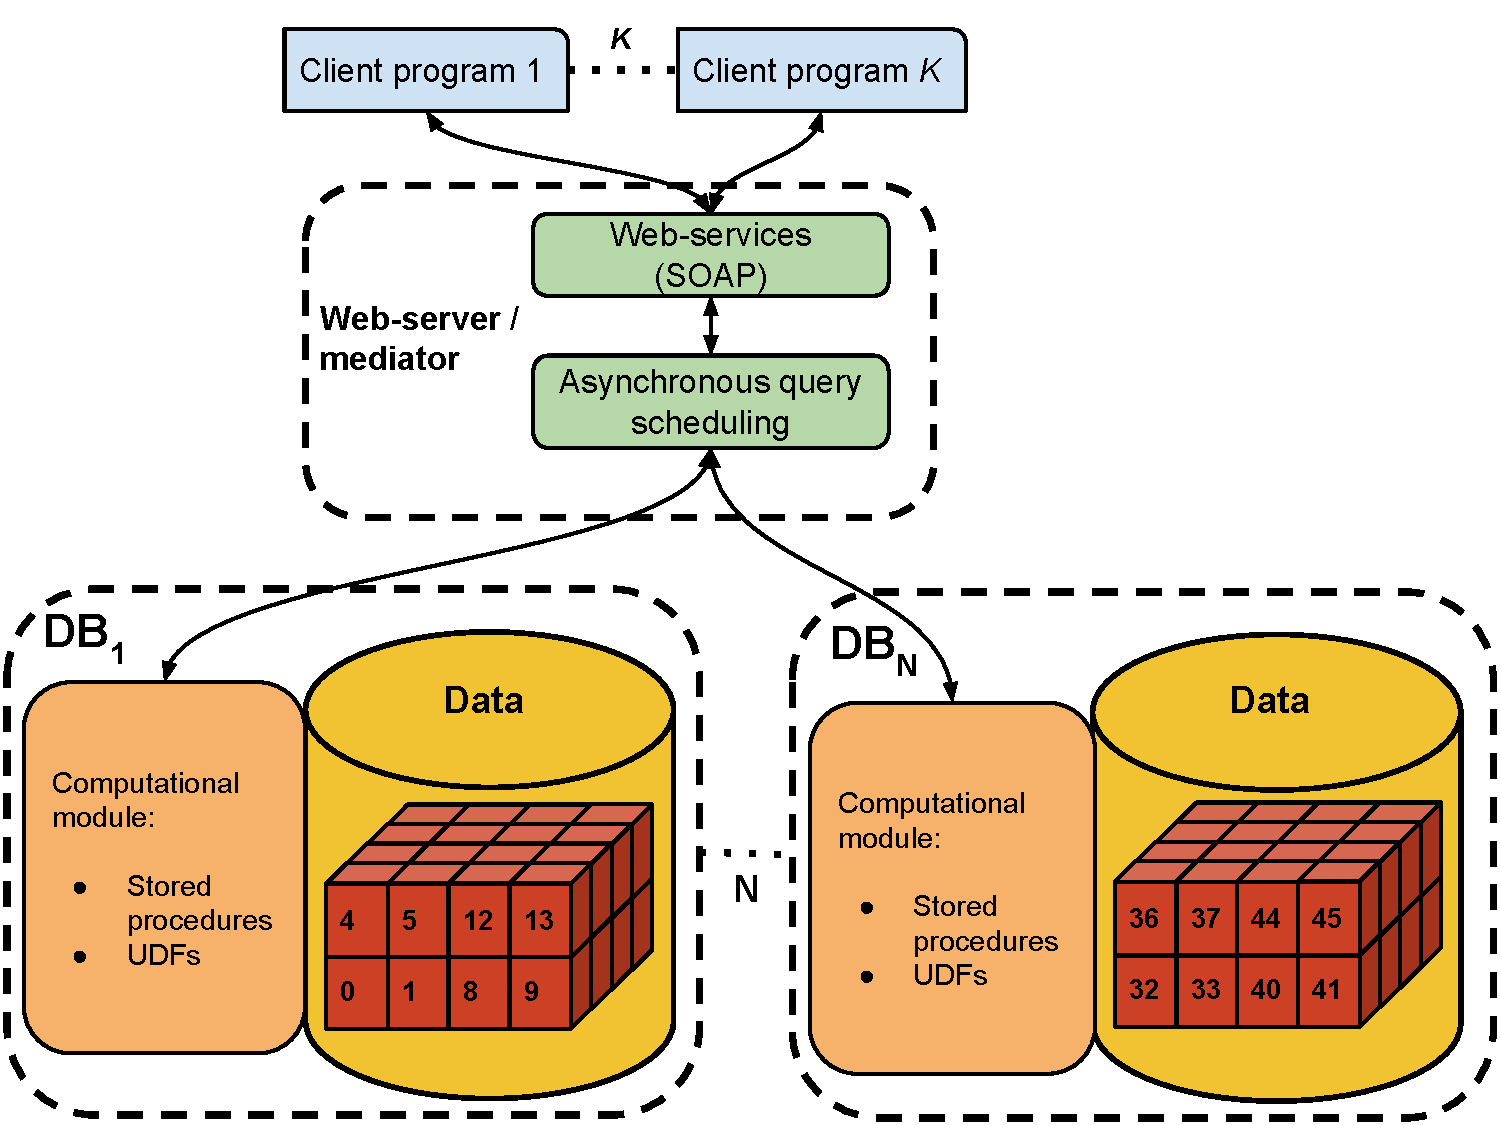
\includegraphics[width=3.35in]{Figures/jhtdb_diagram.pdf}
\caption{Architecture of the JHTDB.}
\label{fig:jhtdb_diagram}
\end{figure}

%What are the key components of my approach and results? Also include any specific limitations.
We present a method for the efficient evaluation of threshold queries over fields derived from the raw vector or scalar fields of the numerical simulation 
stored in the database. 
Our method makes effective use of the cluster resources and achieves high throughput and scalability. 
We exploit the parallelism 
available in the cluster by means of data-parallel execution of the computations. 
%Each computation is distributed across the nodes of the cluster and
%is executed in parallel by several processes within a database node by creating multiple connections to each node. 
We extend the database management system with an
application-aware cache for query results. We build on the idea of an application-aware cache introduced by Lopez et al. \cite{Lopez} and more broadly 
on the concept of semantic caching \cite{Dar}. Rather than caching just data as is the case in system caches and the tree-cache described by Lopez et al.,
we cache the actual results of the computation in a limited version of a semantic cache. 
This leads to query performance improvement of over an order of magnitude.

The contributions of this paper are the following:
\begin{itemize}
\item Computing derived fields of large simulation data on-demand and evaluating threshold queries on them at extreme scale. This provides large
data analytics capabilities that examine entire time-steps of the simulation transparently to the user in a production analysis environment.
\item Achieving this through the combination of existing data management techniques such as data parallelism and semantic caching as well as taking
advantage of heterogeneous scientific cluster architectures (sharded relational DBMS with several SSDs per node).
\item Evaluating the proposed method on data-intensive workloads in a live production environment and showing scalability results on datasets hundreds of terabytes in size.
\end{itemize}

%-The evaluation is computationally limited and embarrassingly parallel, which makes it a good candidate for a GPU implementation.

\section{JHTDB}\label{jhtdb}
Data-intensive architectures and compute clusters built from commodity hardware rely on parallel I/O to multiple disks and high network bandwidth
to achieve high throughput. Such systems have only recently been deployed for the storage of large numerical simulation 
datasets. The virtual laboratories built on these systems make use of relational database system technology to store and manage large array datasets.
Relational database systems however often do not support
all of the functionality that scientists are interested in out of the box. It is either up to the user to develop more sophisticated analysis routines locally or such
capabilities have to be built into the database through user-defined functions or stored procedures. 

The method that we have developed for the evaluation of threshold queries of derived fields was deployed and integrated into the 
Johns Hopkins Turbulence Databases (JHTDB) \cite{Yi, Perlman}. It solves a pressing problem in a production scientific analysis environment, which differs 
from the traditional supercomputing environments and provides large data analytics capabilities transparently to the public. 
The JHTDB, built on top of the GrayWulf and Data-Scope clusters, serves as a public virtual laboratory for
the study of turbulent phenomena. The JHTDB stores several datasets, which are the output of high-resolution numerical simulations of turbulence.
The 3d time-series data are partitioned into small sub-cubes and stored in relational databases distributed across the nodes of the cluster.
Access to the data is provided by means of Web-services and a variety of analysis functions have been
implemented and can be executed through Web-service calls (Fig. \ref{fig:jhtdb_diagram}).
At present the service hosts four datasets, which are available publicly. 
The data are the output of numerical simulations of forced isotropic turbulence, magnetohydrodynamics (MHD), channel 
flow turbulence and homogenous buoyancy driven turbulence.
The total amount of space occupied by the datasets is over 230 TB. 

\begin{figure}
\centering
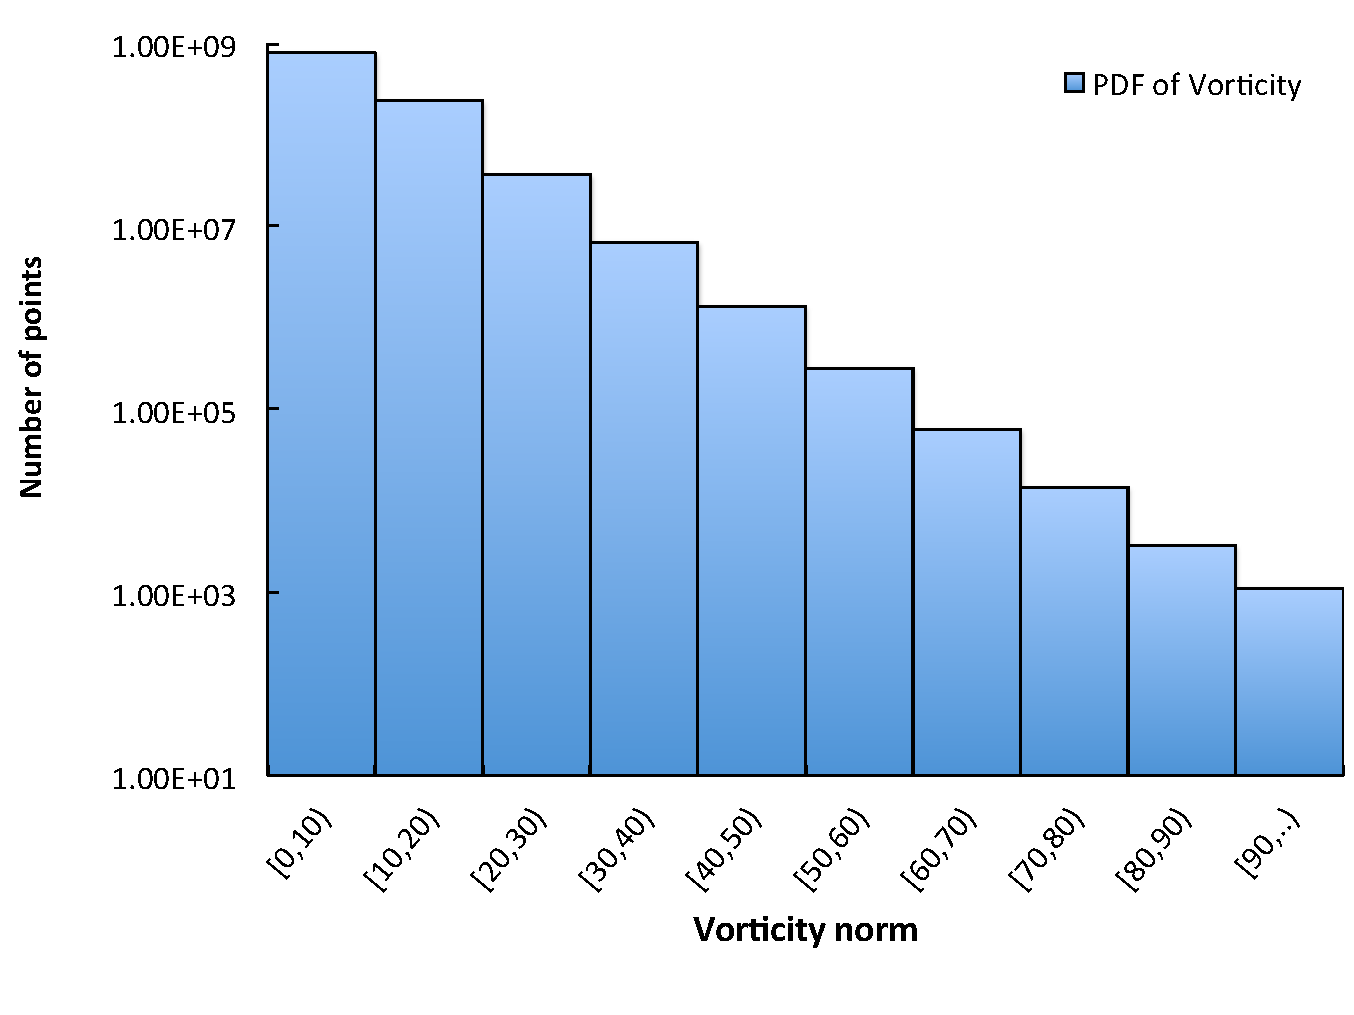
\includegraphics[width=3.35in]{Figures/pdf.pdf}
\caption{Probability density function of the norm of the vorticity field for a representative time-step for the MHD dataset.}
\label{fig:pdf}
\end{figure}

The database nodes are part of the GrayWulf \cite{Szalay} and Data-Scope \cite{DataScope} clusters. Each node
is running Windows Server 2008 and SQL Server 2008 R2. The data for each dataset reside on a regular three-dimensional spatial grid with the
exception of the channel flow data, which has an irregular $y$ dimension. The data are partitioned spatially across 4 to 8
database nodes, and each database node hosts one or more databases. We use the Morton z-order space-filling
curve to distribute the data across nodes and databases \cite{Perlman}. Each time-step is spatially subdivided
into database atoms, which are of size $8^3$. Each such atom is indexed by the time-step, which it belongs to and
by the Morton code of it's lower left corner. This combination of index and data forms a record in the database.
Queries to the data and derived fields, such as derivatives and filtered quantities are evaluated through
stored procedures or user-defined functions implemented in the Common Language Runtime (CLR) framework.

The Web-services are hosted on a front-end Web-server, which handles user requests and hosts the main Web-page portal.
The Web-server acts as a mediator sending the users' requests to the database nodes and initiating their distributed evaluation. 
Each request is broken down into multiple parts based on the spatial layout of the data. Each part is asynchronously submitted for evaluation 
to the database which stores the data needed for the evaluation.
The Web-server assembles the results from the distributed computation and sends them back to the client.

The JHTDB provides a variety of data-intensive analysis routines that are executed on the database nodes. These include interpolation, 
differentiation, particle tracking and spatial filtering. These tasks are often data-intensive and in order to leverage the capabilities of the cluster we
have developed data-driven batch processing techniques for their evaluation \cite{KanovSC11, KanovSC12}. Most of these tasks usually operate on subsets
of the space or a collection of individual target locations within a time-step. 

In contrast, threshold and top-$k$ queries usually have to examine the entire 
data volume of a time-step or a signification portion of it. Furthermore, the data product of threshold queries is much smaller in relation to the amount of 
data that need to be examined. This fact combined with the fact that subsequent queries can reuse 
previously computed results makes the query results suitable to caching. 

\section{Scientific Use Cases}\label{science_use_cases}

%Max vorticity clustering.
One of the applications of thresholding in turbulence is to find the locations of maximum vorticity in a particular time-step or the dataset as a whole.
The locations of maximum vorticity are usually associated with the most intense vortices in the dataset and often have interesting and complex
reconnection events associated with them. 
Once obtained from the service, these locations can be clustered in both 3d and 4d. This allows scientists to examine their evolution with the flow
and make subsequent analysis queries as needed in order to study these events. The relationship between different ``worms'' (see Figure \ref{fig:max_vort_cluster}) that connect and reconnect
at those locations is of the most interest.

\begin{figure*}[t]
\centering
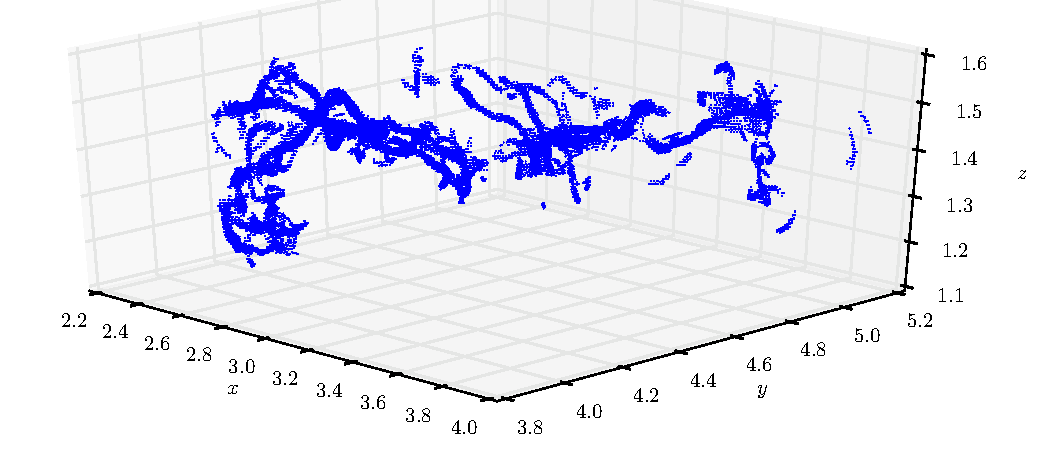
\includegraphics[width=7in]{Figures/most_intense_cluster_alt.pdf}
\caption{3D (single time-step) cut through the 4D cluster containing the most intense event.}
\label{fig:max_vort_cluster}
\end{figure*}

The vorticity is computed from the velocity field by taking its curl:
\begin{align}
\vec{\omega} &= \vec{\nabla} \times \vec{v} = \left( \frac{\partial}{\partial x}, \frac{\partial}{\partial y}, \frac{\partial}{\partial z} \right) 
\times \nonumber \left( v_x, v_y, v_z \right)\\
&= \left( \frac{\partial v_z}{\partial y} - \frac{\partial v_y}{\partial z}, \frac{\partial v_x}{\partial z} - \frac{\partial v_z}{\partial x}, 
\frac{\partial v_y}{\partial x} - \frac{\partial v_x}{\partial y} \right).
\label{eq:curl}
\end{align}
We use finite differencing methods of
different orders for the evaluation of the curl. For example, with 4th-order centered finite differencing each partial derivative is evaluated from the 4
adjacent grid node values as follows:  
\begin{align} 
\left.\frac{df}{dx}\right|_{x_n} = &\frac{2}{3\Delta x}[f(x_{n+1})-f(x_{n-1})]\nonumber\\ 
&-\frac{1}{12\Delta x}[f(x_{n+2})-f(x_{n-2})],
\end{align}
where $f$ denotes any one of the three components of the velocity and $\Delta x$ is the width of the grid in the $x$ direction. The partial derivatives
along $y$ and $z$ are computed in the same fashion. 
Figure \ref{fig:pdf} shows the distribution of the values of the norm of the vorticity field in the MHD dataset for a representative time-step. This is indicative 
of how the values are distributed in the dataset as a whole.
This coarse view of the data can be used by scientists to guide the selection of threshold values.

Figure \ref{fig:max_vort_cluster} shows the most intense event observed in the MHD dataset. The locations of maximum vorticity in the dataset were clustered
in this case in 4d using a friends-of-friends algorithm. It is interesting to note that the cluster containing the most intense event in the entire dataset develops
from nothing (i.e. it does not appear in the first few time-steps) and it takes less than the timespan stored in the database for it to develop. 
%The timespan stored is equal to about one large eddy turnover time. 
%It is not clear whether a different more intense event could emerge from an existing
%cluster if the timespan stored was larger. 
Figure \ref{fig:max_vort_cluster} also shows that most interactions between worms are not simple. 
There are several worms interacting in a complex way at the same time. Similar type of analysis and the fact that the entire time history of the simulation
is available in a database cluster, which provides built-in sophisticated analysis routines revealed flux-freezing breakdown in MHD turbulence \cite{Eyink},
showing why solar flares last minutes rather than the millions of years that theory would predict.

In addition to obtaining the regions of largest vorticity, there is substantial interest in studying the regions with highest values for other fields, such as
the second and third velocity gradient invariants ($Q$ and $R$). These invariants are scalar quantities whose values contain information about the 
topology of the flow and the rates of vortex stretching and rotation. In MHD, finding the locations with largest values for the electric current
can lead to new insights into the development of the most intense reconnection events of magnetic field sheets in the simulated plasma. Similarly to
the vorticity, the electric current is derived from the magnetic field by taking its curl. The list of fields of interest, on which scientists would like to perform 
threshold queries certainly does not stop here and is indicative of how valuable this functionality is in the study of turbulence and fluid dynamics.

\section{Threshold Query Evaluation}

Threshold queries of derived fields submitted to the JHTDB are evaluated using a data-parallel execution strategy and the query results are 
cached in an application-aware cache, which is a limited version of a semantic cache. 
The evaluation strategy for queries that do not hit the cache is driven by the spatial partitioning of the data across the nodes of the cluster.

{\bf Derived fields computation:} The databases store only the raw field data from the simulation (e.g. velocity, pressure, magnetic field etc.). However,
the threshold queries of most interest to science users produce all locations where the values of a \emph{derived} field are above a given threshold. Thus, the
derived field in question has to be computed from the raw data first. For most derived fields of interest, this computation has local support. It has an 
associated localized kernel of computation around each grid node. Therefore, the value of the derived field at each grid node depends on the value of the
stored field at all of the grid locations, which are part of the kernel of computation. 

{\bf Distributed data-parallel execution:} In most cases threshold queries operate over an entire time-step. Each such query is subdivided by 
the mediator into queries submitted to
each of the database nodes. Each node evaluates the query over the data that it has stored locally. Only a small amount of data along the boundary
need to be requested from adjacent nodes. The size of the band of data that may not be available locally is equal to a kernel half-width. 
Such a band is needed on each of the sides of the box forming the domain of the computation.  
The data are read into memory and the particular field requested is computed at each of the locations on
the grid. The same strategy applies when utilizing multiple processes per node. The norm or absolute value of the derived field at each location is compared 
against the specified threshold and if the value is higher, it is maintained along with
the spatial coordinates of the location in a list.

We impose a limit on the maximum number of locations that can be returned as a result of a threshold query in order to prevent having to return
the entire time-step or a significant fraction of it for queries with thresholds that are set too low. Currently this limit is set conservatively to $10^6$ locations, 
which is sufficient to examine a time-step in detail. In the case of the vorticity, the values above 8 times the root mean square value, 
which is about $25\%$ of the maximum, are contained within $2.6\times10^5$ points in each time-step. Figure \ref{fig:points_7rms} shows all the points 
in a single time-step with values above 7 times the root mean square value. There are $2.4\times10^5$ points in the figure.
Given that we are interested in extreme events, obtaining the locations with values even within $50\%$ of the maximum would be sufficient. 
At the same time this also limits the amount of data that have to be returned to the user over the network as well as the amount of
data that have to be cached. Users receive an error message notifying them if their request has a threshold that is set too low. If a user
is interested in obtaining more data he or she can request the values of the derived field directly. Alternatively, if they are interested in the density distribution
of values they can examine the probability density function (e.g. Fig. \ref{fig:pdf}), which is computed using a similar strategy to threshold queries.

\begin{figure}
\centering
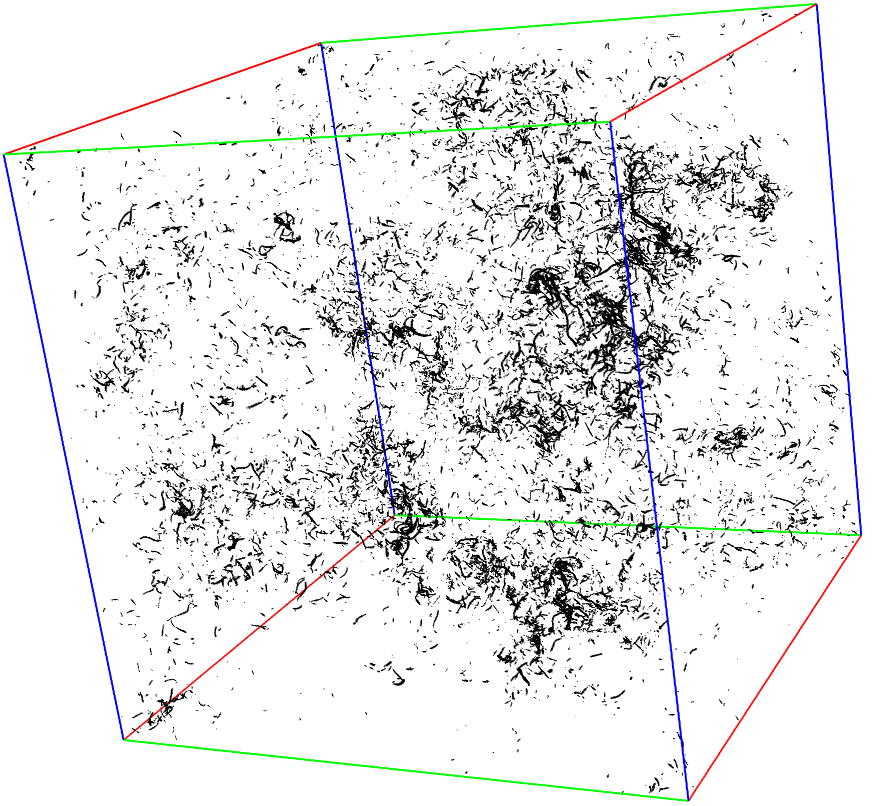
\includegraphics[width=3.35in]{Figures/points_7rms.png}
\caption{Points with values above 7 times the root mean square value of the vorticity for a single time-step.}
\label{fig:points_7rms}
\end{figure}

\begin{figure}
\centering
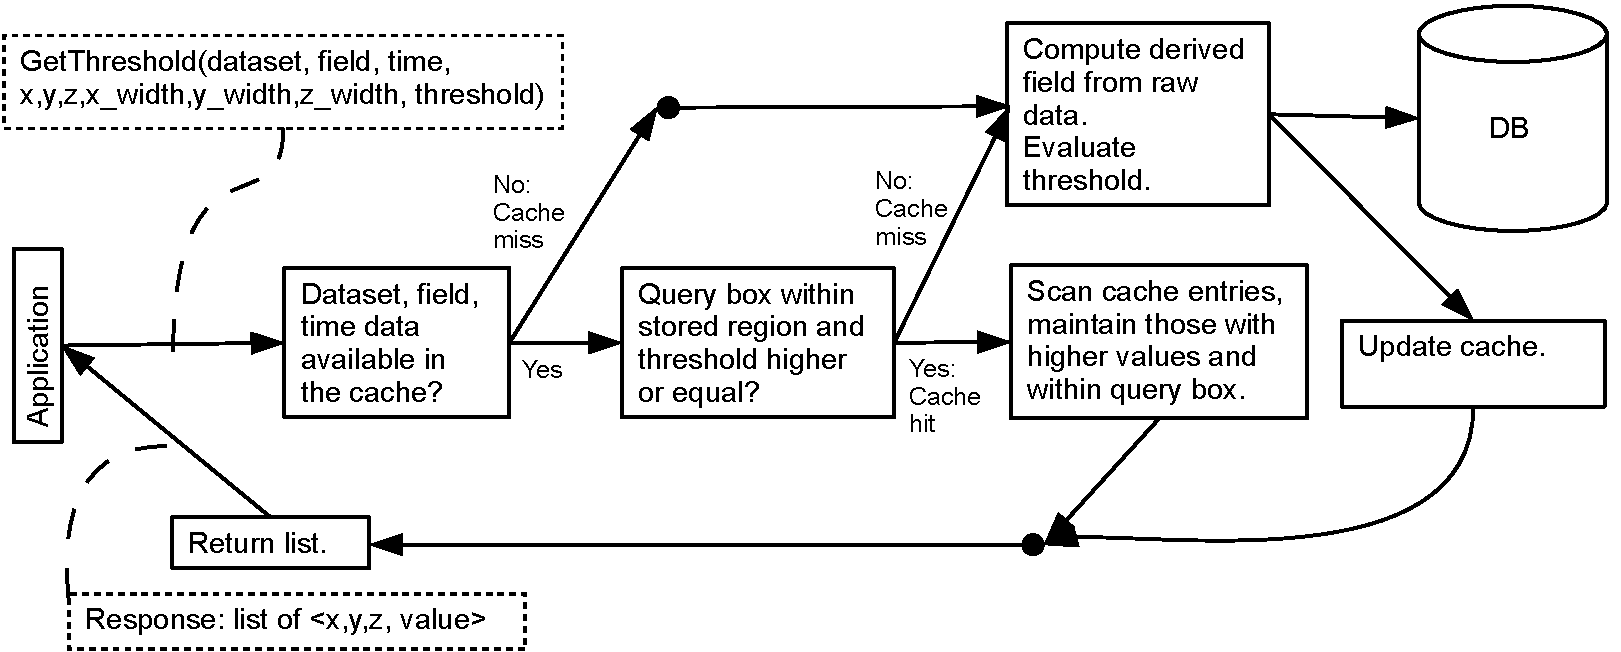
\includegraphics[width=3.35in]{Figures/cache_diagram.pdf}
\caption{Distributed evaluation of threshold queries and architecture of the application-aware cache. 
Each database node has local cache tables, which reside on solid-state drives attached to the node.}
\label{fig:cache_diagram}
\end{figure}

{\bf Application-aware cache for query results:} A central part of the evaluation strategy for threshold queries that we have developed is the 
introduction of an application-aware cache
for query results (Fig. \ref{fig:cache_diagram}). The results of these queries are small compared to the amount of data that need to be examined and the
results can be used to answer subsequent queries as long as they are within the same region and specify the same or higher threshold. Each database node 
has a local cache. Cache entries are indexed by the field, time-step, spatial region and the threshold requested. We use a least recently
used cache replacement policy. All modifications of and queries to the cache are executed within a transaction with snapshot isolation level to
avoid dirty-reads or an inconsistent view of the cache. 

Caching the query results
preserves the computational effort in addition to substantially reducing I/O. The cached data are for the particular derived field that was queried
and not the raw data of the simulation fields.
Thus, we do not have to derive the requested field from the raw data for 
queries that hit the cache. This results in a substantial improvement in query performance as we only have to scan
a small set of data and do not need to perform any additional computation.

Not all query results are suitable to caching. Most of the queries submitted to the JHTDB other than threshold queries request data at a collection of target
locations. Given that there are $1024^4$ possible locations for three of the datasets and $6*1024^4$ locations for the channel-flow dataset the chance of
reuse for the results of these queries is extremely small. This is why the cache currently stores only the results of threshold queries. Nevertheless, it can 
easily be extended to cache the results of other query types as well if that becomes advantageous.

The cached query results are stored in a table in the database and the overall size of the cache is limited by the amount of available SSD disk space, not memory.
Given a limit of $\sim$$10^6$ points per time-step for a threshold query, the space required to cache the maximum number of points including the index
space and database overhead is $\sim$40MB. 
Therefore for a dataset containing 
1024 time-steps, as is the case for the isotropic turbulence and MHD datasets part of the JHTDB, a cache size of 40GB is sufficient to cache the query
results for threshold queries of a derived field over the entire dataset. In contrast, computing and materializing a scalar derived field for the entire dataset will
require $\sim$5TB (15TB for vector fields).

\begin{algorithm}
\caption{Get points above threshold using cache}\label{alg:cache_lookup}
\begin{algorithmic}[1]
\Require Dataset $d$, Field $f$, Timestep $t$, Threshold $k$, Query box $q = [x_l,y_l,z_l,x_u,y_u,z_u]$
\Procedure{GetThreshold}{}
\State $points \gets List()$
\State $updateCache \gets false$
\State $query \gets \text{SELECT * FROM cachedb..cacheInfo}$
\Statex[4] $\text{WHERE dataset = {\it d} AND field = {\it f}}$
\Statex[4] $\text{AND timestep = {\it t}}$
\State $command \gets SqlCommand(query)$
\State $reader \gets command.ExecuteReader()$
\If {$reader.HasRows()$}
\State $k_s \gets reader[``threshold"]$ \Comment{Stored threshold}
\State $start \gets reader[``startIndex"]$
\State $end \gets reader[``endIndex"]$
\State $ordinal \gets reader[``ordinal"]$
\If {$k \ge k_s \And q \in \text{[start, end]}$}
\State $\textit{query} \gets \text{SELECT * FROM cachedb..cacheData}$
\Statex[4] $\text{WHERE cacheInfoOrdinal = {\it ordinal}}$
\State $command \gets SqlCommand(query)$
\State $reader \gets command.ExecuteReader()$
\While{reader.Read()}
\State $location \gets reader[``zindex"]$
\State $norm \gets reader[``dataValue"]$
\If {$norm \ge k \And location \in q$}
\State $\textit{points.Add(new Point(location, norm))}$
\EndIf
\EndWhile
\Else
\State $updateCache \gets true$
\EndIf
\Else
\State $updateCache \gets true$
\EndIf
\If {$updateCache$}
\State $\text{Retrieve data covering {\it q} from DB.}$
\ForAll{$p \in q$}
\State{Compute $f$ at $p$.}
\If{$\| f(p) \| \ge k$}
\State $\textit{points.Add(new Point(p, $\| f(p) \|$))}$
\EndIf
\EndFor
\State{Update cacheInfo and cacheData tables.}
\EndIf
\State{\Return $points$}
\EndProcedure
\end{algorithmic}
\end{algorithm}

The entire cache is comprised of two database tables. The {\it cacheInfo} table stores metadata for the cached entries. It stores information about the
dataset, field, time-step, start and end coordinates of the spatial region examined and the threshold value used. The {\it cacheData} table stores the locations
of all of the grid points, for which the field queried has a norm higher than the specified threshold. The {\it cacheData} table is foreign key constrained with
the ordinal of the {\it cacheInfo} table. This allows us to quickly find a record in the {\it cacheInfo} table and retrieve all of the cached entries using an index
lookup.

{\bf Overall execution of threshold queries:} Algorithm \ref{alg:cache_lookup} illustrates the process of obtaining all points with norms of the specified field
above the given threshold from the database in the presence of a cache. 
The mediator submits a query to each of the database nodes storing the raw data
asynchronously. Each node begins evaluation of the query by executing Algorithm \ref{alg:cache_lookup}. 
First a cache lookup is performed.
If the data for the requested field, time-step and spatial region
are available in the cache and if the specified threshold is higher than the one stored in the cache the query can be answered from there. The records are
retrieved from the cache and the ones that have a higher value are returned to the mediator and subsequently back to the user. If the data stored in the
cache have a higher threshold than the one requested the cache needs to be updated. Similarly, if the cache does not have an entry for the specified 
parameters the query needs to be evaluated from the raw data. In those cases the raw data are read into memory with data along the boundary requested
from adjacent nodes as needed. The specified field is derived at each location on the grid and the norm or absolute value of the field is
compared against the threshold. The locations where the values are higher than the threshold need to then be stored in the cache. If the cache does not
have enough space for the new records, space is freed up by removing the least recently used data across all quantities. Reading from, updating or
modifying the cache is done within a transaction with snapshot isolation level. Snapshot isolation allows us to avoid locking the tables that serve as the 
cache for each transaction. This provides for a higher degree of parallelism and avoids any potential deadlocks from queries running in parallel.

\section{Experimental Results}
We evaluate the developed method for the execution of threshold queries to large numerical simulation datasets with the goal of analyzing the 
benefits and overhead from the introduction of the application-aware cache. We also analyze the scaling properties of the method. Finally, we show
that an integrated method that performs the evaluation on the database nodes near the data is several orders of magnitude faster than the
user requesting the derived filed of interest from the database and evaluating the threshold locally.

%\vspace{10 pt}
\subsection{Experimental Setup}
The experiments were run on the production database nodes of the JHTDB through a development Web-server hosting the Web-services. We used
the MHD dataset (Sec. \ref{jhtdb}) for the experimental runs. This dataset is partitioned across 4 database nodes according to spatial regions in the
Morton z-order. 
The database nodes are 2.66 GHz dual quad-core Windows 2008 servers with SQL Server 2008 R2 and 24 GB of memory. Each node has 24 2TB 
SATA disks arranged as a set of four RAID-5 arrays. The database files are striped across the nodes and their associated disk
arrays. The tables storing the data are partitioned spatially along contiguous ranges of the Morton z-curve and the data for each partition reside in one
database file. 

\begin{figure}
\centering
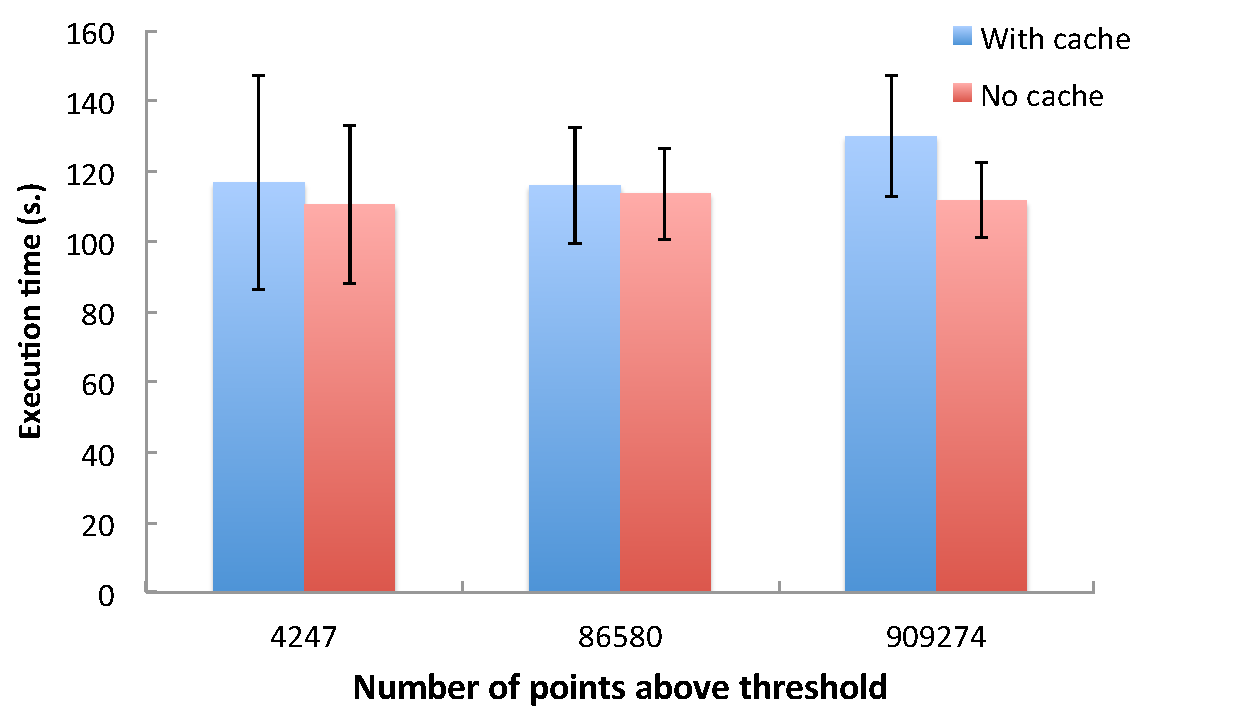
\includegraphics[width=3.35in]{Figures/cache_overhead.pdf}
\caption{Execution time for threshold queries at different threshold levels compared with the execution time of the same queries in the
absence of a cache.}
\label{fig:cache_overhead}
\end{figure}

For this evaluation we looked at the performance of threshold queries to the vorticity field. The vorticity field is representative of derived fields that
have to be computed from the stored data. It is defined as the curl of the velocity field.
As described in section \ref{science_use_cases}
thresholding the vorticity field is important in the study of fluid dynamics and obtaining the locations of maximum vorticity can lead to new insights into
the development of the most intense vortices observed in the dataset. 

\begin{figure*}
\centering
\subfigure[Scale-up with multiple processes per node]{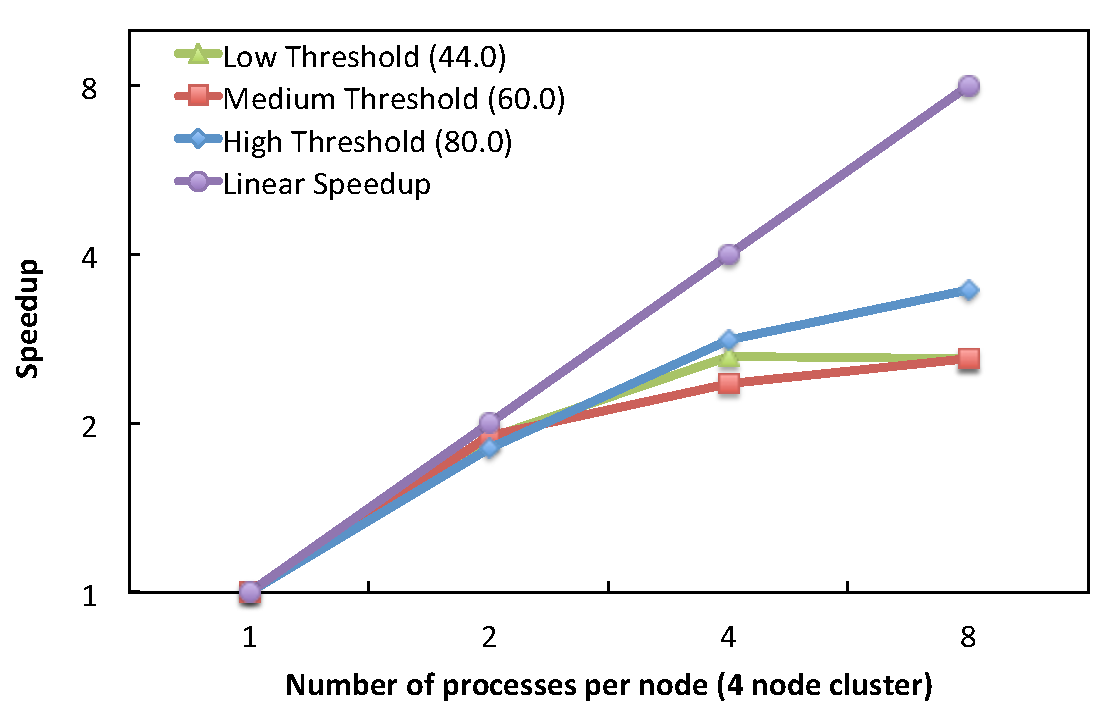
\includegraphics[width=3.35in]{Figures/scaleup.pdf}\label{fig:scaleup}}
\subfigure[Scale-out to multiple nodes]{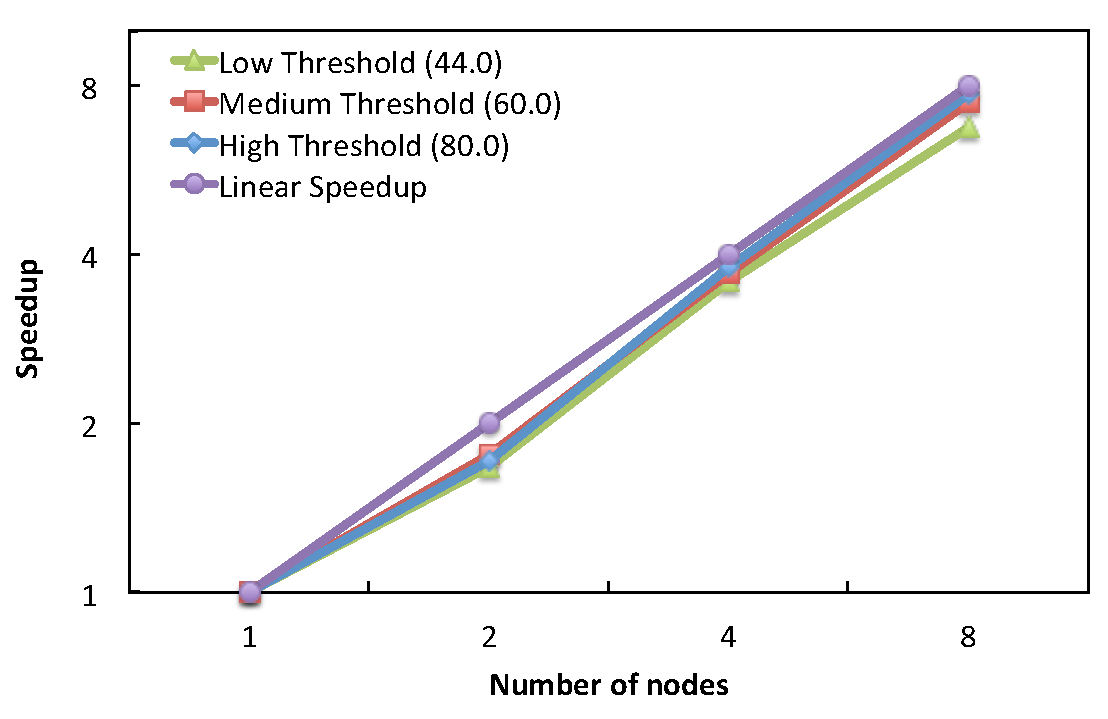
\includegraphics[width=3.35in]{Figures/scaleout.pdf}\label{fig:scaleout}}
\caption{Execution time for threshold queries at different threshold levels -- high, medium and low. The scale-up evaluation was performed 
utilizing 1-8 processes per server on a 4-node cluster. The scale-out evaluation was performed on 1 through 8 nodes.}
\label{fig:scaling}
\end{figure*}

\subsection{Evaluation of cache effectiveness}

The central part of the strategy that we have developed for the evaluation of threshold queries of derived fields is the application-aware cache, which
stores the results of these queries. We first evaluate the overhead associated with the introduction and maintenance of the cache. Figure
\ref{fig:cache_overhead} compares the execution time of queries in the absence of a cache with the execution time of the same queries, which interrogate
the cache first (blue and red bars in the figure). The execution times are also shown in Table \ref{tab:cache_effectiveness}. 
For these experiments we requested
the locations with norms of the vorticity above thresholds at different levels. We refer the reader to Figure \ref{fig:pdf}, which shows the distribution of values of
the norm of the vorticity field in the MHD dataset to get an appreciation of the different threshold values used in the experiments. 
For the first set the threshold was set high (80.0) and only $\sim$4,300 points 
(or 0.0004\% of all points) were above the threshold. For the second set a medium threshold (60.0) was chosen and $\sim$87,000 points 
(or 0.0081\% of all points) were above the threshold. Finally, a low threshold (44.0) was chosen for the last set and there were $\sim$900,000 points 
(or 0.0847\% of all points) above the threshold. For each set a random
time-step was chosen and the queries were run against that time-step. The measurements were taken from the point of view of the end user. 

As we can see from the results shown in Figure \ref{fig:cache_overhead} the overhead associated with querying the cache first is minimal, 
less than 3\% and within the margin of error.
The cache was initially populated by executing several hundred unrelated queries and contained several million entries.
During the ``cache-miss" runs cache entries for the particular time-step queried were dropped before each run, making sure that each query would
produce a cache miss and would have to be evaluated from the raw data. 
The execution times were averaged over 10 runs.
We utilized 4 processes per database node for the evaluation of each query. 
The method shows stable running time across different time-steps and threshold levels in the absence of a cache and during cache misses.
The running time increases slightly only because of the larger result set that has to be returned to the user.
%Additionally, the method shows stable running time across different time-steps and threshold levels even with cache
%misses. The slight increase in the running time that can be observed is due to the larger result set that has to be returned to the user.

\begin{table}[h]
\centering
\begin{tabular}{|c|c|c|c|c|} \hline
\multirow{2}{0.5in}{Vorticity threshold} & \multirow{2}{0.5in}{Points above threshold} & \multicolumn{3}{|c|}{Average Running time (s.)}\\ \cline{3-5}
& & No cache & \parbox[t]{0.55in}{With cache (miss)} & \parbox[t]{0.55in}{With cache (hit)} \\ \hline
80.0 & 4247 & 97.1 & 100.2 & 0.5\\ \hline
60.0 & 86580 & 113.7 & 115.9 & 1.2\\ \hline
44.0 & 909274 & 111.6 & 115.0 & 9.1\\ \hline
\end{tabular}
\caption{Effectiveness of caching.}
\label{tab:cache_effectiveness}
\end{table}

Cache hits reduce the running time of threshold queries by over an order of magnitude as shown in Figure \ref{fig:cache_overhead} and
Table \ref{tab:cache_effectiveness}. This is because we do not have to compute the requested derived
field from the raw data, which eliminates the associated I/O. Only the cache entries need to be looked-up, which is substantially less data
than the raw vector or scalar field data. For the queries with large result sets it is actually the network time taken to transfer the results to the user that 
dominates the overall execution as opposed to the I/O or computation time as we show later.
Cache hits are evaluated by first warming up the cache by submitting the same set of threshold queries of the vorticity field as before. We then submit
several more unrelated queries with different time-steps and threshold values in order to pollute the cache. Finally, we issue the original set of queries and 
measure their running times. Let us focus on the query
with low threshold, which returns $\sim$900,000 points. Given that valid threshold values are limited to those that result in no more than 1,000,000 points
it is likely that all subsequent queries to this time-step will result in a cache hit as their threshold is likely to be equal or higher than the cached one.

\subsection{Scaling and Distributed Evaluation}
The evaluation of threshold queries of derived fields from the raw data is both I/O and computationally bound. These queries examine the entire data
volume of a simulation time-step and are, therefore, good candidates for a data-parallel distributed evaluation. 
Our data-parallel implementation exhibits good vertical and nearly ideal horizontal scaling as shown in Figure \ref{fig:scaling}. 
For the scale-up experiments (Fig. \ref{fig:scaleup}), we used the same
queries and threshold values as for the runs shown in Figure \ref{fig:cache_overhead} and Table \ref{tab:cache_effectiveness} 
but with varying number of processes per node. Cache entries for the
time-step queried were again dropped before each run in order to evaluate the scaling properties of the computation of the derived field from the stored data.
The computations for all of 
the derived fields of interest (such as the vorticity) at each grid point need data from adjacent grid points only. Therefore, each node of the cluster is able to
compute the derived field from data available locally with only a small amount along the boundary of each region having to be retrieved from adjacent nodes.
Each computation is independent and embarrassingly parallel. This allows us to make use of multiple processes per node and scale out to
multiple database nodes.

We observe nearly a two times speedup when going from a single process per node to two processes per node (Fig. \ref{fig:scaleup}). 
The speedup diminishes to 1.4 times when going to 4 processes and little speedup is 
observed with 8 processes per node. This is due to several factors. Each node has 2 CPUs and a total of 8 cores, which need to run operating system and other SQL Server
processes as well. The experiments were run on the live production database nodes, which were also servicing other user queries. Additionally, SQL
Server already utilizes parallelism to perform most of the I/O. Finally, due to the data-parallel approach to the evaluation of these queries the data atoms along
the boundary of each region are requested by multiple processes. Nevertheless, running with 4 processes per node is nearly 2.6 times faster when
compared to running with a single process.

The scale-out experiments show a nearly perfect linear speedup as the evaluation is distributed to an increasing number of database nodes 
(Fig. \ref{fig:scaleout}). For these experiments we issued queries with the same threshold levels as before to a cold cache. We utilized a single process per
database node to evaluate the horizontal scaling of the computation. The evaluation benefits not only from the additional computational resources with
the addition of database nodes to the cluster but also from the increased memory size. The data needed for the computation of each derived field are
read into memory and the larger memory size means that there is less contention with other system and application processes and it is less likely that
virtual memory needs to be used. SQL Server also benefits from a larger buffer pool, which reduces the I/O time.

\begin{figure}
\centering
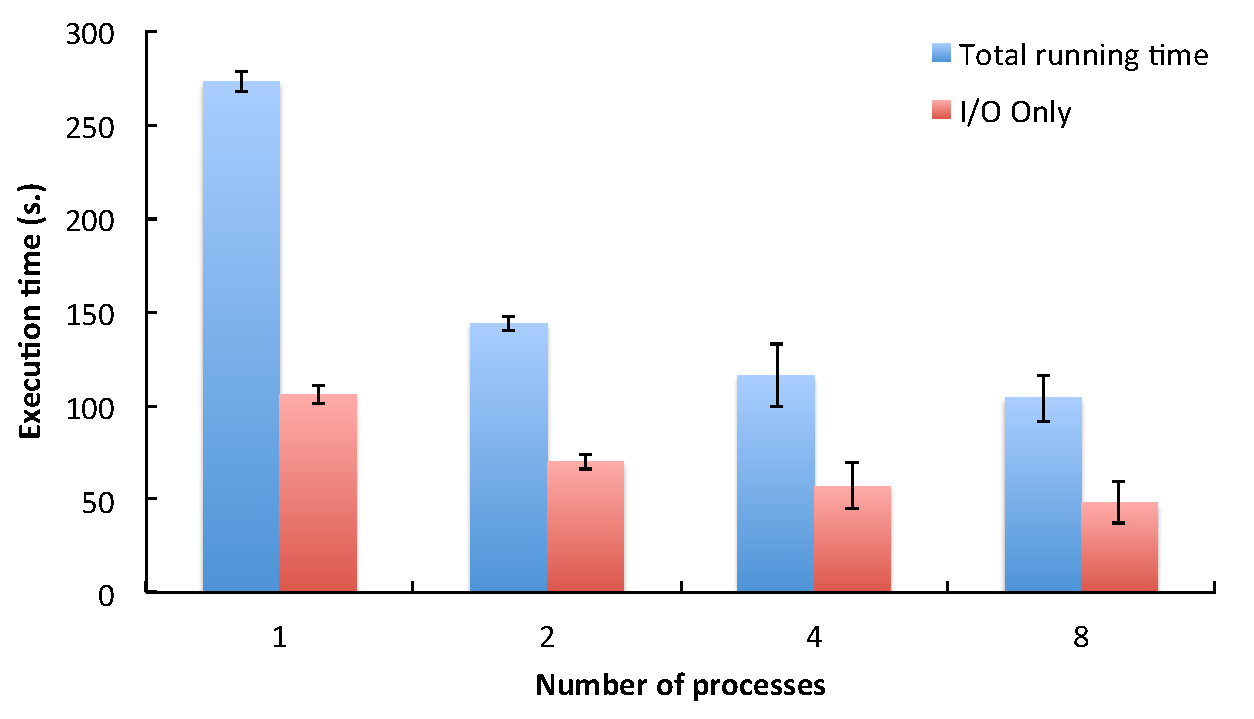
\includegraphics[width=3.35in]{Figures/io_comparison.pdf}
\caption{Execution time for threshold queries evaluated utilizing different number of
processes per server compared with the time taken to perform the I/O only.}
\label{fig:io_comparison}
\end{figure}

\begin{figure*}
\centering
\subfigure[Vorticity]{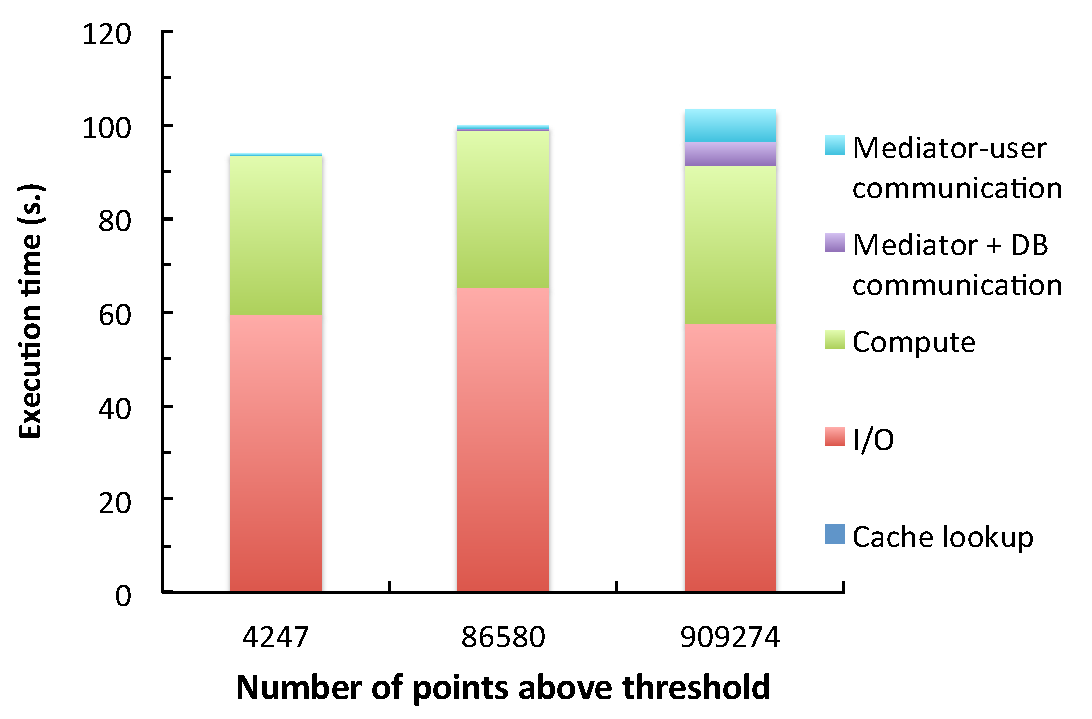
\includegraphics[width=2.2in]{Figures/vorticity_breakdown.pdf}\label{fig:vorticity_breakdown}}
\subfigure[Q-criterion]{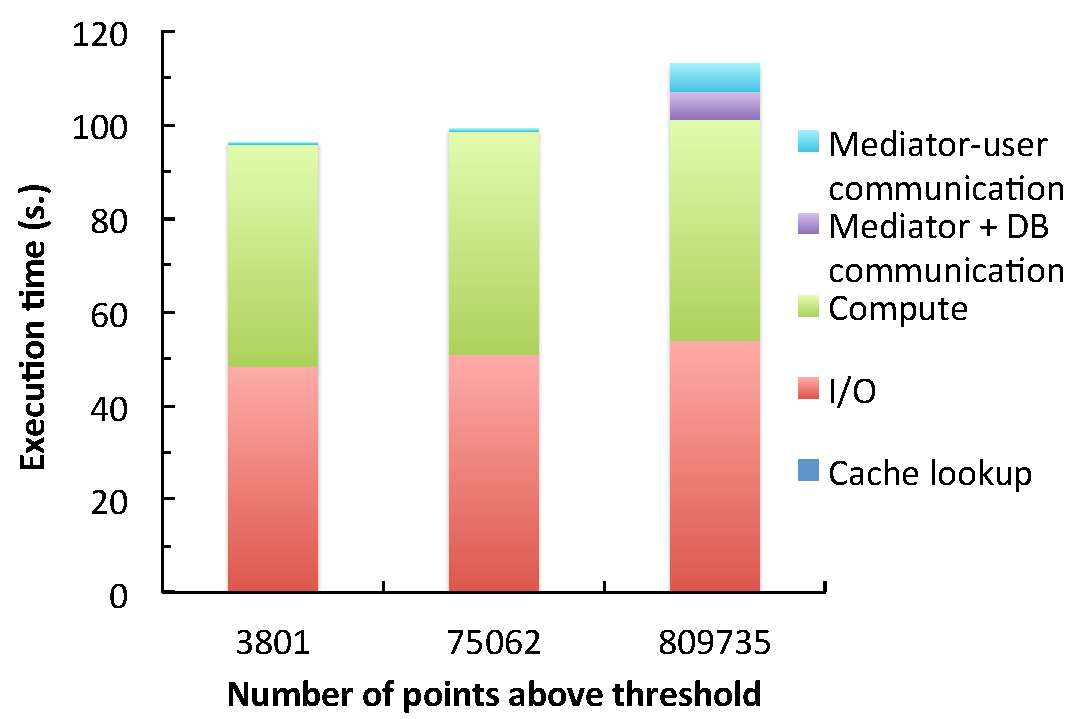
\includegraphics[width=2.2in]{Figures/q_breakdown.pdf}\label{fig:q_breakdown}}
\subfigure[Magnetic field]{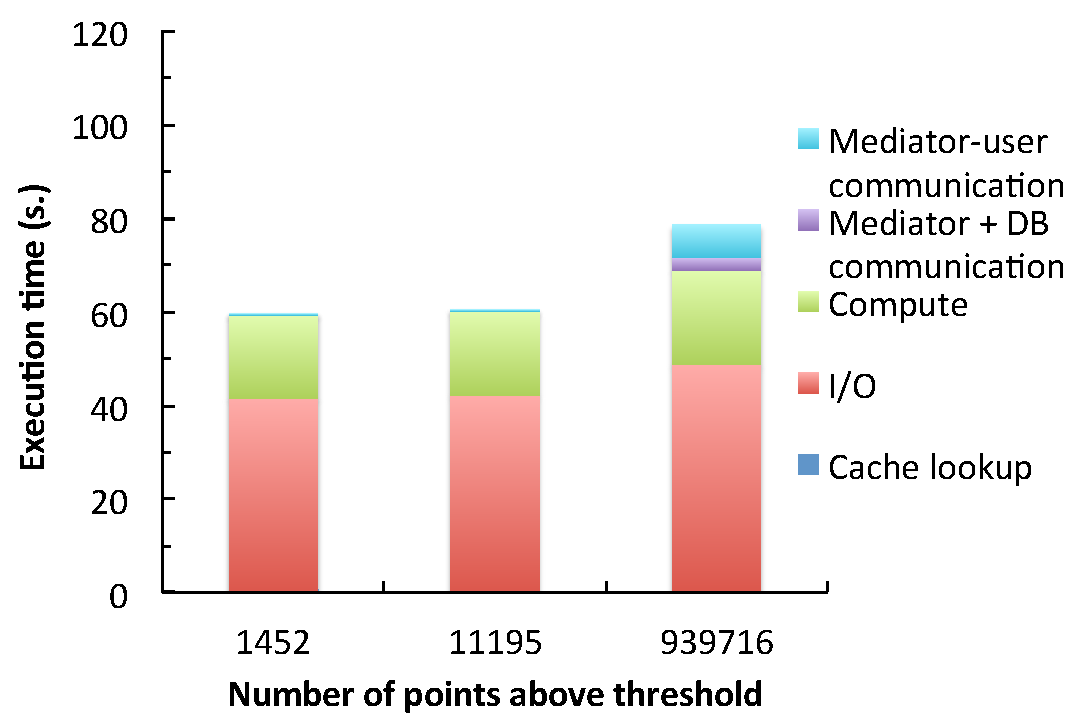
\includegraphics[width=2.2in]{Figures/magnetic_breakdown.pdf}\label{fig:magnetic_breakdown}}
\subfigure[Vorticity (cache hit)]{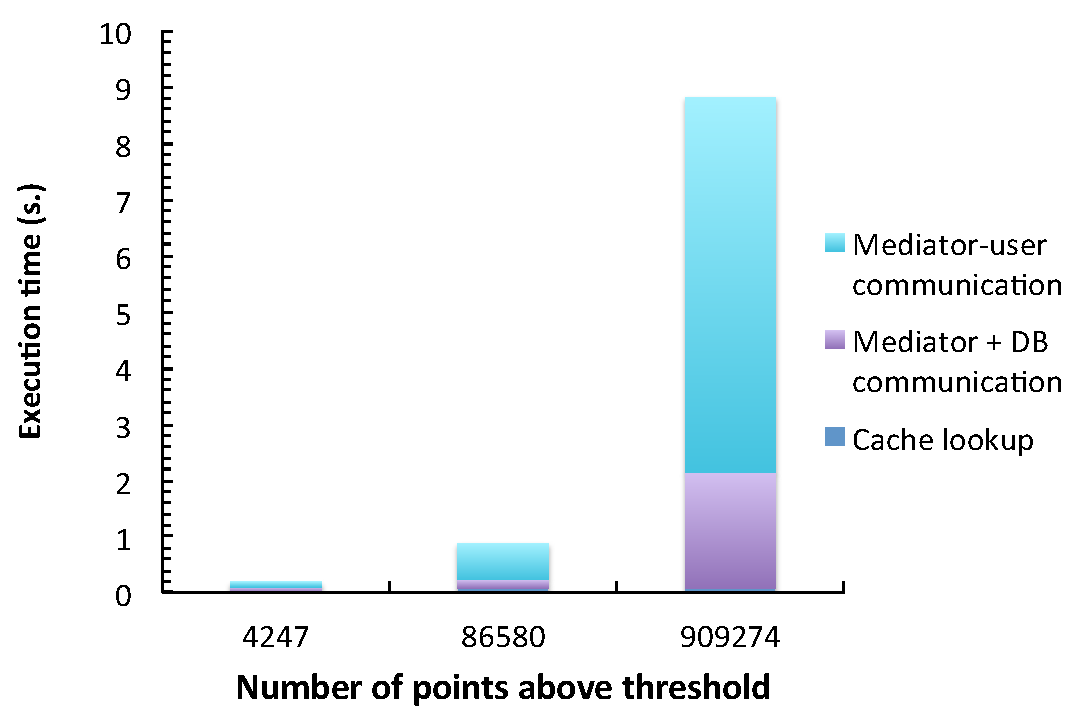
\includegraphics[width=2.2in]{Figures/vorticity_breakdown_cachehit.pdf}\label{fig:vorticity_breakdown_cachehit}}
\subfigure[Q-criterion (cache hit)]{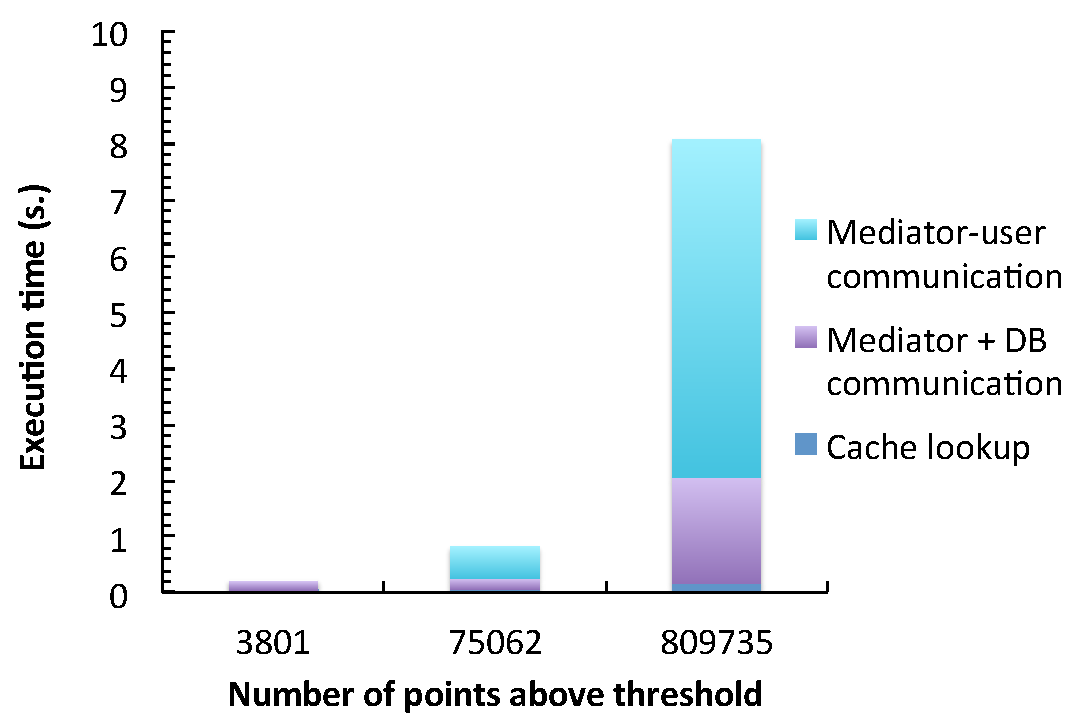
\includegraphics[width=2.2in]{Figures/q_breakdown_cachehit.pdf}\label{fig:q_breakdown_cachehit}}
\subfigure[Magnetic field (cache hit)]{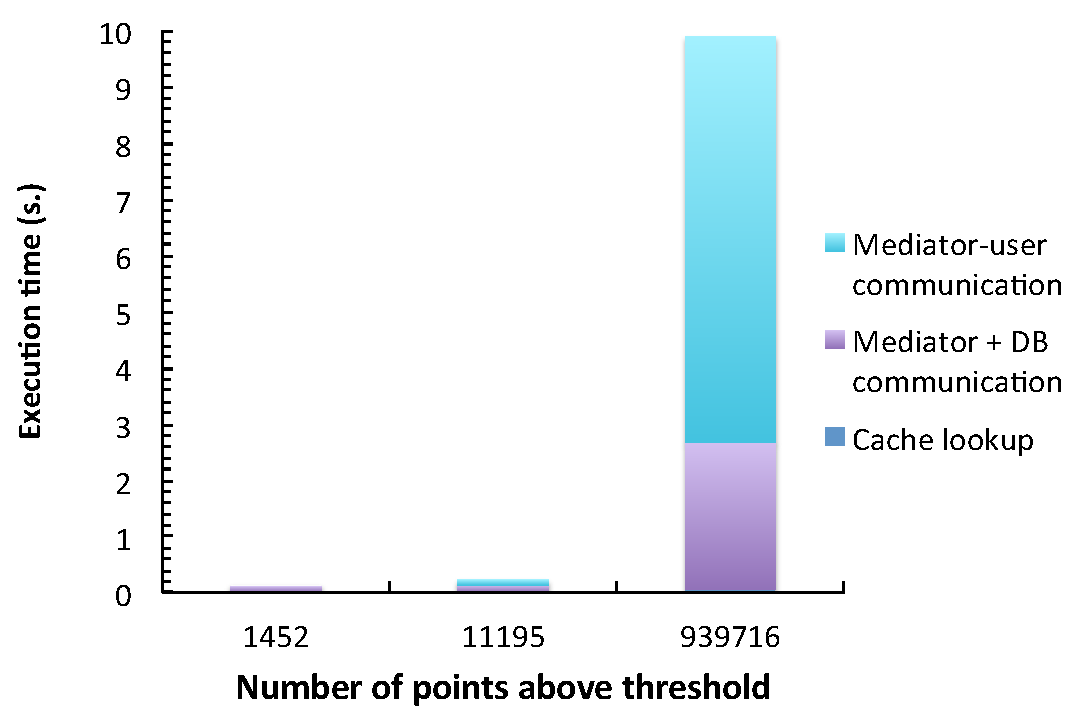
\includegraphics[width=2.2in]{Figures/magnetic_breakdown_cachehit.pdf}\label{fig:magnetic_breakdown_cachehit}}
\caption{Breakdown of the execution time for threshold queries requesting different fields and at different threshold levels -- high, medium and low.}
\label{fig:breakdown}
\end{figure*}

As expected, we observe even weaker speedup when the queries perform nothing but I/O and the number of processes per node is increased.
Figure \ref{fig:io_comparison} compares the running time of the queries with a medium threshold and executed with varying number of processes per 
node with
the time taken to perform the I/O only. The I/O time is about half of the total running time for these queries. SQL Server already makes use of parallelism
internally and the data have to be retrieved from the same set of disks. Nevertheless, the I/O time does decrease with additional processes, this is because
the data reside in a partitioned table and the data in each partition are placed in a separate file on one of the disk arrays. Depending on how the data
requests are scheduled in SQL Server this allows for the disks arrays to be driven in parallel. Additionally, with more processes per node the data can
also be consumed faster. It is worth noting that the total running time for the queries evaluated with 4 or 8
processes is about the same as the time it takes to perform the I/O only with a single process.

So far we have presented the effectiveness of evaluating threshold queries of derived fields on the database cluster storing the raw simulation data. The 
data-parallel computation of the derived fields allows us to evaluate a threshold query over
an entire $1024^3$ time-step part of a 20TB dataset in less than two minutes. The introduction of an application-aware cache for the query results of these
queries reduces this time to several seconds when there is a cache hit. In contrast, one of our science collaborators reported that his evaluation of this
functionality performed locally would take over 20 hours to complete. 
To perform the evaluation locally the user requests the derived field of interest from the database by submitting multiple queries over
subregions of a time-step. This is necessary as requesting a derived field over an entire time-step will overload the network. Derived fields may have even
more components than the scalar or vector field stored in the database. For example, the velocity gradient (needed for the computation of the vorticity) has 9
components compared with the 3 components of the velocity. Given a single-precision floating-point representation, this makes the velocity gradient of an
entire time-step at least 36GB in size. A Web-service request will be much larger due to the overhead of wrapping the data in an xml format. After the
field of interest is obtained locally the user has to threshold it to get the final result, which is reasonably fast, but discards most of the data that have been
requested to yield a small in size result. 

\subsection{Evaluation of Additional Fields}
The data-parallel evaluation of threshold queries shows stable execution time for different derived fields in addition to the different threshold levels and
time-steps queried. The execution times depend on the complexity of the computation needed to evaluate the particular derived field requested. Figures 
\ref{fig:vorticity_breakdown}, \ref{fig:q_breakdown}, \ref{fig:magnetic_breakdown} show a breakdown of the execution time of threshold queries of different
derived fields, which are evaluated from the raw data and a cold cache using 4 processes per node on a 4 node cluster. Almost the entire time is spent
performing the I/O and computation associated with the derived field requested. 

The vorticity field and the Q-criterion have similar I/O requirements as they
have the same kernels of computation and are both derived from the velocity gradient. The vorticity has 3 components and its computation only examines
6 of the 9 components of the velocity gradient, which are also examined in pairs (see Eq. \ref{eq:curl}). On the other hand, even though the Q-criterion is a
scalar value, it is computed through a non-linear combination of all 9 of the components of the velocity gradient. This means that the velocity gradient has
to be computed at each grid location before the Q-criterion is evaluated, which is reflected in the increased computation time that we observe for the
Q-criterion. The magnetic field is one of the raw fields of the magnetohydrodynamics dataset that are stored in the database. Therefore, there is no
additional computation needed to derive it from the data, every data point has to be simply compared with the threshold level specified. This is why the 
computation time is much smaller compared to the queries for the vorticity and the Q-criterion. The I/O time for the magnetic field is also smaller. This is
because its kernel of computation is a single point and therefore there are no additional data along the boundary that have to be requested from adjacent 
nodes. In that case all of the data needed are available locally for each database node.

In all of these cases, the time taken to interrogate the cache is negligible. The mediator time to distribute the queries and assemble the results as well as the
time to transfer them to the user are also substantially smaller than the I/O and computation times. As expected they increase proportionally to the number
of points in the result set.

It is interesting to note that the time taken to perform a cache lookup is relatively small even in the case of a cache hit as can be seen in Figures 
\ref{fig:vorticity_breakdown_cachehit}, \ref{fig:q_breakdown_cachehit} and \ref{fig:magnetic_breakdown_cachehit}. This is because the cache tables reside on
SSDs attached to each database node (see Fig. \ref{fig:cache_diagram}) and retrieving the data is always done through a clustered index lookup.
In the cases of a cache hit, the majority of the time is spent simply transferring the results from the database nodes to the mediator and then back to the user.
These times remain more or less constant between the cases of cache misses and cache hits (top row and bottom row of Fig. \ref{fig:breakdown}).
Caching the results of threshold queries
effectively preserves the I/O and computational effort spent during their initial evaluation and results in over an order of magnitude speedup for all the
different fields requested as we can see in Figure \ref{fig:breakdown}.

\section{Related Work}
Only select few database systems offer support for arrays as first-class citizens. Even fewer provide the fault-tolerance, scalability and availability guarantees 
necessary for a system managing multi-terabyte datasets in a production setting. This is part of the reason why we have chosen to represent the array
data in the JHTDB as a collection of binary large objects in a relational DBMS and perform the array manipulation tasks necessary at the application level.
The systems that provide
support for arrays and aim to handle large array data efficiently are RasDaMan \cite{Rasdaman}, SciDB \cite{Scidb} and MonetDB/SciQL \cite{Sciql}. RasDaMan
partitions raster objects into tiles, which are stored in a traditional relational database system. This approach is similar to how the numerical simulation data
are handled in the JHTDB. RasDaMan provides RasQL \cite{Rasql}, which is a SQL-92 based query language for the manipulation of raster images. SciDB
is an array database system build from the ground up. Array attributes are partitioned vertically and each attribute array is decomposed into overlapping
chunks. SciDB provides a declarative Array Query Language (AQL) and an Array Functional Language (AFL). Users can create arrays with named
dimensions with AQL and make use of the functional operators defined in AFL, such
as SLICE, SUBSAMPLE, SJOIN, FILTER and APPLY. SciQL's focus is on language design and integration with SQL:2003 syntax and semantics. It is implemented
within the MonetDB framework \cite{MonetDB}.

Database systems support rollup queries, including top-$k$ queries, but in most cases these
queries apply only simple linear score functions on the attribute values of individual records.
Additionally, many top-$k$ query evaluation techniques rely on the score functions being monotone in order to perform early pruning (see \cite{Ilyas} for a
survey of top-$k$ evaluation strategies).
This is an assumption that we cannot make for the functions used to compute all the different possible derived fields of interest in fluid mechanics.
Even approaches that aim to work with general score functions \cite{Deshpande, Xin} assume that the function operates on the attributes of a single record.
In contrast, our approach performs a stencil kernel computation at each grid location in order to obtain the value of a \emph{derived} field at that location and
examines the vector or scalar array data at all neighboring locations, which
are within the kernel of the computation. The functions used to derive the field may even be non-linear.
Finally, a top-$k$ approach may not be suitable in the cases where scientists are interested in performing threshold queries at different time-steps as the
same threshold level will produce different number of points in the result set for different time-steps.

The processing of top-$k$ queries has been studied extensively in the context of distributed and relational database systems. A survey of different techniques
in the case of centralized processing is given in \cite{Ilyas}. In the case of distributed processing different approaches focus on horizontally 
\cite{Balke, Vlachou} or vertically \cite{Cao, Chaudhuri, Guntzer, Marian, Michel} distributed data. None of these approaches deals with array data stored in
a relational database system. Zhao et al. propose an algorithm for the processing of top-$k$ queries in large-scale distributed environments called BRANCA
\cite{Zhao}. They build on the idea of semantic caching \cite{Ren} and make use of branch caches, which store results of previous top-$k$ queries with respect 
to the data stored on each server. The caching mechanism that we use is similar in that regard, but the queries that are evaluated in our system operate on
derived fields, which are computed at each location by accessing data from a surrounding region. The queries described in \cite{Zhao} operate over the 
attributes of individual records only using simple linear score functions.

A{\ss}falg et al. introduce the concept of threshold queries in time-series databases \cite{Asfalg}. Their definition of threshold queries differs from the threshold
queries described in this paper. They are concerned with determining the time-series, which exceed a user-defined threshold at time frames similar to
the time-series specified in the query. Thus, their definition of threshold queries is concerned with the temporal relationship between the time-series
stored in the database (usually one dimensional sequence of measurements) and the time-series given in the query. In contrast, our approach focuses on
reporting all of the spatial locations of a multidimensional field where the norm or absolute value of the field exceeds a user prescribed threshold.

In a system called the tree cache, Lopez et al. \cite{Lopez} make use of a small application-aware cache to reduce access time to large datasets stored on
disk. The tree cache stores individual octants of octree datasets and exploits application-specific information to determine which octants to cache and to 
perform query reordering. This work has inspired the use of an application-aware cache for the evaluation of threshold queries. In contrast to the tree cache,
we do not cache raw data objects, but rather query results. Caching query results preserves the computational effort in addition to reducing I/O, which has a
much bigger impact on query performance and substantially reduces the size of the cache. Additionally, the cache that we introduce resides on disk rather 
than in memory, which greatly increases its potential size. Lopez et al. also explore approximate querying through aggregation, which can be fairly easily
supported by our system but is of limited use as scientists performing threshold queries are usually interested in obtaining the exact locations where a field is 
at its highest values.

Sampling approaches \cite{Sidirourgos, Nirkhiwale} offer an alternative to the on-demand computation of derived fields and the evaluation of threshold queries
on them. The goal of both techniques is to not return large data volumes, but focus on the most intense events and interesting regions in the dataset. 
The computation of the derived fields is carried out on the nodes of the database cluster and takes a look at the dataset as a whole, while the user obtains only
a small subset of the data, where the derived field in question is above the prescribed threshold. Sampling approaches can potentially omit some locations and
while useful for generating initial impressions may not be suitable if the exact locations where a field is at its highest values are desired.

Andrade et al. \cite{Andrade} describe a database system and an optimization framework build on the concept of \emph{active semantic caching}. An
active semantic cache aims to fully or partially reuse cached query results or aggregates through automated transformations of these aggregates. Similarly
to our work they focus on real scientific data-analysis applications. The method that we have developed for the evaluation of threshold queries complements
the active semantic caching approach and could be used in that framework. Our work has focused on extending a relational database system (Microsoft's SQL
Server) as opposed to designing a new database system from the ground up as described by Andrade et al. \cite{Andrade}.

\section{Conclusions and Future Work}

We have presented an efficient strategy for the evaluation of threshold queries of derived fields in large numerical simulation datasets. 
The thresholded fields are derived from the stored simulation data in a distributed data-parallel manner. The computations
scale with the cluster resources and are performed on the database nodes, where the data are stored. This new capability allows researches to quickly
obtain and focus on regions of special interest even if they lack the computing capabilities or data transfer rates necessary to examine entire time-steps
or large parts of the entire dataset. 

We have introduced an application-aware cache for the query results of threshold queries. Cache hits reduce query running times by over an order of
magnitude. The cache adds minimal overhead during the evaluation of queries even if there is
a cache miss and has modest storage requirements. The cache is represented as a set of database tables and resides on disk rather than in memory. 
Each database node has local cache tables, which allows the cache to scale-out as the cluster grows.

The introduction of an application-aware cache for query results lays the groundwork for the creation of a landmark database. Such a database can store the 
locations of the highest vorticity regions in the dataset or more broadly regions of interest and their associated statistics.

The Web-services approach to archived numerical simulation datasets provides public access to high quality simulation data to anyone with an internet
connection. The Web-services methods can be called from any modern programming language and we provide C, Fortran and Matlab client libraries for the
JHTDB. The evaluation of each query submitted through a Web-service call is carried out on the nodes of the database cluster by means of a stored
procedure
or a user-defined function that has been implemented and deployed to handle these requests. This allows us to fine-tune the execution of these procedures
and handle all requests transparently to the user. However, this approach also has drawbacks. Adding new functionality means adding to a long list of 
Web-service calls and requires substantial implementation effort. In the case of threshold queries the stored procedure performing the evaluation must have
an implementation for each derived field of interest even though the execution is handled by the same Web-service call. 

In the future, we plan to develop
declarative and graphical user interfaces that will allow users to combine existing building blocks and perform computations that have not been explicitly
implemented. Additionally, we plan on deploying a server-side computing environment for users similar to the CasJobs service for the Sloan Digital Sky Survery \cite{LiThakar}. In such an environment users can run queries in batch mode and save their results in a personal database called MyDB, which 
resides on the servers near the data.
This will allow for much greater flexibility in the type of computations that can be performed in addition to substantially decreasing the network overhead.

\section{Acknowledgments}
The authors would like to thank the Turbulence Database Group at Johns Hopkins University as well as three anonymous reviewers for
their insightful comments and suggestions. This work is supported in part by the National Science Foundation
under Grants CDI-II: CMMI 0941530 and OCI-108849 and Johns Hopkins University's Institute for Data Intensive Engineering \& Science.

\bibliographystyle{abbrv}
\bibliography{paper} 

\end{document}
